% Chapter 5

\chapter{Experimentations \& Validation} % Main chapter title

\label{Chapter5} % For referencing the chapter elsewhere, use \ref{Chapter5}

\section{Pushing tests with Pepper}

\paragraph{} Before trying to implement the algorithm on the actual Pepper robot, the first thing to do was to check if it actually could push obstacles with certainty as to the result of the manipulation. More precisely, we needed to know what kind of movable obstacles we could move with confidence in the results, and how to position the robot relatively to the obstacle for the push action to succeed.

\subsection{Pepper robot characteristics}

\paragraph{} The Pepper robot is a mass-produced humanoid service robot by the company Softbank Robotics\footnote{Softbank Robotics website: \url{https://www.softbankrobotics.com/emea/en}}. For sensors, it is equipped with:

\begin{itemize}
  \item Two sonars, at the front and the back (Figure \ref{fig:sonars}), that allow to detect obstacles in the close vicinity, but not to characterize their geometry (with them, the robot can only know that an obstacle is in front or behind, at a certain distance, but cannot discern its form),
  \item Three laser sensing units at the front and the sides (Figure \ref{fig:lasers}), that allow it to roughly detect the form of nearby obstacles (only 15 points per sensor at a maximum distance of 3 meters). It is to be noted that, together, these three units do not cover the surroundings of the robot at 360 degrees, but leave very big blind spots,
  \item Three bumpers at each corner of its triangular base, to detect collisions that may occur,
  \item A 2D RGB camera on its forehead (Figure \ref{fig:2d_camera}), that allows it to do image recognition tasks or simply filming its environment,
  \item A 3D RGBD camera\footnote{Asus XTion Camera: \url{https://www.asus.com/us/3D-Sensor/Xtion_PRO_LIVE/}} in its head (Figure \ref{fig:3d_camera}), behind the eye lenses, that allow it to construct a 3D point cloud of the obstacles in front of where its face is turned, which can be used to cover part of laser units blind spots,
  \item An inertial measurement unit that allows it to know its orientation.
\end{itemize}

\paragraph{} In particular, three other sensors are especially meant for interaction with humans:

\begin{itemize}
  \item A touchscreen (also an actuator) on its chest, for complex interactions,
  \item Two directional microphones on the top of its head that can be used to detect where a noise is coming from or interact vocally,
  \item Various touch sensors over its body, including on the hands, that allow it to interact physically.
\end{itemize}

\begin{figure}[H]
\centering
\begin{subfigure}{.48\textwidth}
  \centering
  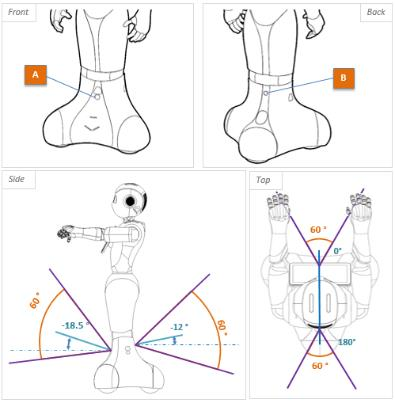
\includegraphics[width=\linewidth]{Figures/Pepper_Robot/sonars.jpg}
  \caption{Sonars}
  \label{fig:sonars}
\end{subfigure}\hspace*{\fill}
\begin{subfigure}{.48\textwidth}
  \centering
  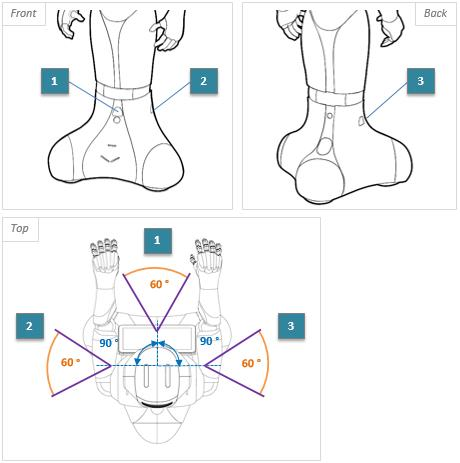
\includegraphics[width=\linewidth]{Figures/Pepper_Robot/lasers.jpg}
  \caption{Lasers}
  \label{fig:lasers}
\end{subfigure}
\caption{Positioning and field of vision of Pepper's sonars and lasers}
\label{fig:sonars_lasers}
\end{figure}

\begin{figure}[H]
\centering
\begin{subfigure}{.48\textwidth}
  \centering
  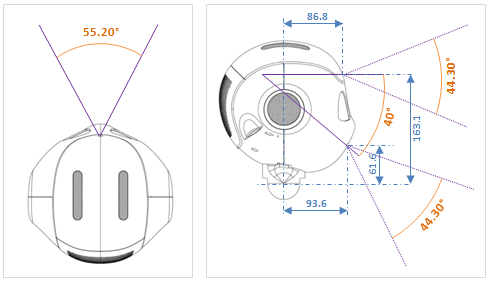
\includegraphics[width=\linewidth]{Figures/Pepper_Robot/2d_camera.png}
  \caption{2D Camera}
  \label{fig:2d_camera}
\end{subfigure} \hspace*{\fill}
\begin{subfigure}{.48\textwidth}
  \centering
  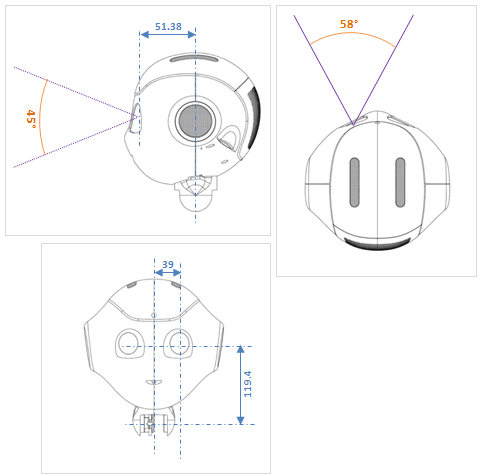
\includegraphics[width=\linewidth]{Figures/Pepper_Robot/3d_camera.png}
  \caption{3D Camera}
  \label{fig:3d_camera}
\end{subfigure}
\caption{Positioning and field of vision of Pepper's cameras}
\label{fig:cameras}
\end{figure}

\paragraph{} As for actuators, Pepper is equipped of omnidirectional wheels that allow it to turn in place and not be forced to face the direction it is translating toward. Two motors allow it to fold its body a little, just above the base and at the hips, but not enough for it to be able to touch the ground with its arms. Two motors allow the head to move forward/backward and turn left or right (but not for a full turn). Finally, it has two articulated arms including fingers, that are mainly meant for interactions with humans, but not for lifting large or heavy obstacles.

\paragraph{} All these characteristics are important, because they condition the way we can implement a navigation algorithm.

\subsection{On experimentation repeatability with ROS and Pepper}

\paragraph{} We mentioned at the beginning of our work that the \groupname \, uses ROS\footnote{ROS, the Robot Operating System, website: \url{http://www.ros.org/}} to program Pepper. ROS is a robotics middleware, and, in fact, not an operating system. It provides a high-level abstraction of hardware while still allowing for low-level device control, task distribution over a network capabilities, and most importantly, a message-passing system between processes, that allows a great diversity of programs written in many different languages to still be able to talk to one another. It also brings a package management system, that is coupled with the packaging system of the GNU/Linux distribution Ubuntu\footnote{Official website: https://www.ubuntu.com/}, allowing for plug-and-play capabilities for new software components.

\paragraph{} Experimentation reproducibility has been a long standing problem in robotics \parencite{guglielmelli_research_2015, bonsignorio_toward_2015}. As an example, in the entire studied corpus presented in Chapter \ref{Chapter2}, no paper links to actual code or a Virtual Machine (VM) to test the simulations. Even using a standard like ROS does not make an experiment done with it reproducible in itself, since one needs the exact same version of ROS, the same GNU/Linux distribution and version, the same libraries, the same robotic platform with the same peripherals (when using a real robot), \dots To solve this problem at least on a software level, in the last few years, the ROS foundation financed efforts toward using ROS inside of Docker\footnote{https://www.docker.com/} containers \parencite{white_ros_2017}, a technology close to the idea of a VM, but lighter and faster, since it does not isolate the running code as much as a VM.

\paragraph{} For us to be able to actually execute our experiment, and for allowing others to reproduce it more easily, we have therefore built upon this work to propose a Docker container configuration that allows to connect to the Pepper Robot and reproduce the following experiment on any Linux-Enabled system. All instructions required to set it up are available in the following git repository: \\ \url{https://github.com/Xia0ben/rosdocked-kinetic-pepper}.

\subsection{Experiment}

\paragraph{Objective} We want to test several movable obstacles types to see if and how Pepper could manipulate them with confidence as to the results.

\paragraph{Hypothesis} Given the round nature of Pepper's base front, we suppose that light obstacles and obstacles with wheelcasters could be moved. We suppose that placing the robot at the center of the obstacle's side, and pushing in a perpendicular direction to it gives the most repeatable results.

\paragraph{Protocol}

\begin{itemize}
  \item We start a Docker container to connect to the robot, following the instructions in the \href{https://github.com/Xia0ben/rosdocked-kinetic-pepper}{previously presented repository}.
  \item Position Pepper at the beginning of the test line with an obstacle at its base in a given configuration (for each obstacle, we at least test the middle of the obstacle's side, and if results were encouraging, also positions at the border of the obstacle where the robot would have two, then one contact points). Take photos from the side (wide + close angle), top (only close angle) and front (wide + close angle), see Figure \ref{fig:experimental_setup}.
  \item Start a video take from side and front wide angles, and send the following command to tell Pepper to go forward for only about 1.5 meters
  \begin{minted}{bash}
  \$ rostopic pub /cmd_vel -1 geometry_msgs/Twist\
  '{linear:  {x: 0.5, y: 0.0, z: 0.0}, angular: {x: 0.0,y: 0.0,z: 0.0}}'\
  && sleep 1 &&\
  rostopic pub -1 /cmd_vel geometry_msgs/Twist\
  '{linear:  {x: 0.0, y: 0.0, z: 0.0}, angular: {x: 0.0,y: 0.0,z: 0.0}}'
  \end{minted}
  \item Take photos from the side (wide + close angle), top (only close angle) and front (wide + close angle) to notice the drift from the robot's trajectory.
  \item Reposition Pepper, position the tested obstacle, and restart the experimentation.
\end{itemize}

\begin{figure}[H]

\begin{subfigure}{0.20\textwidth}
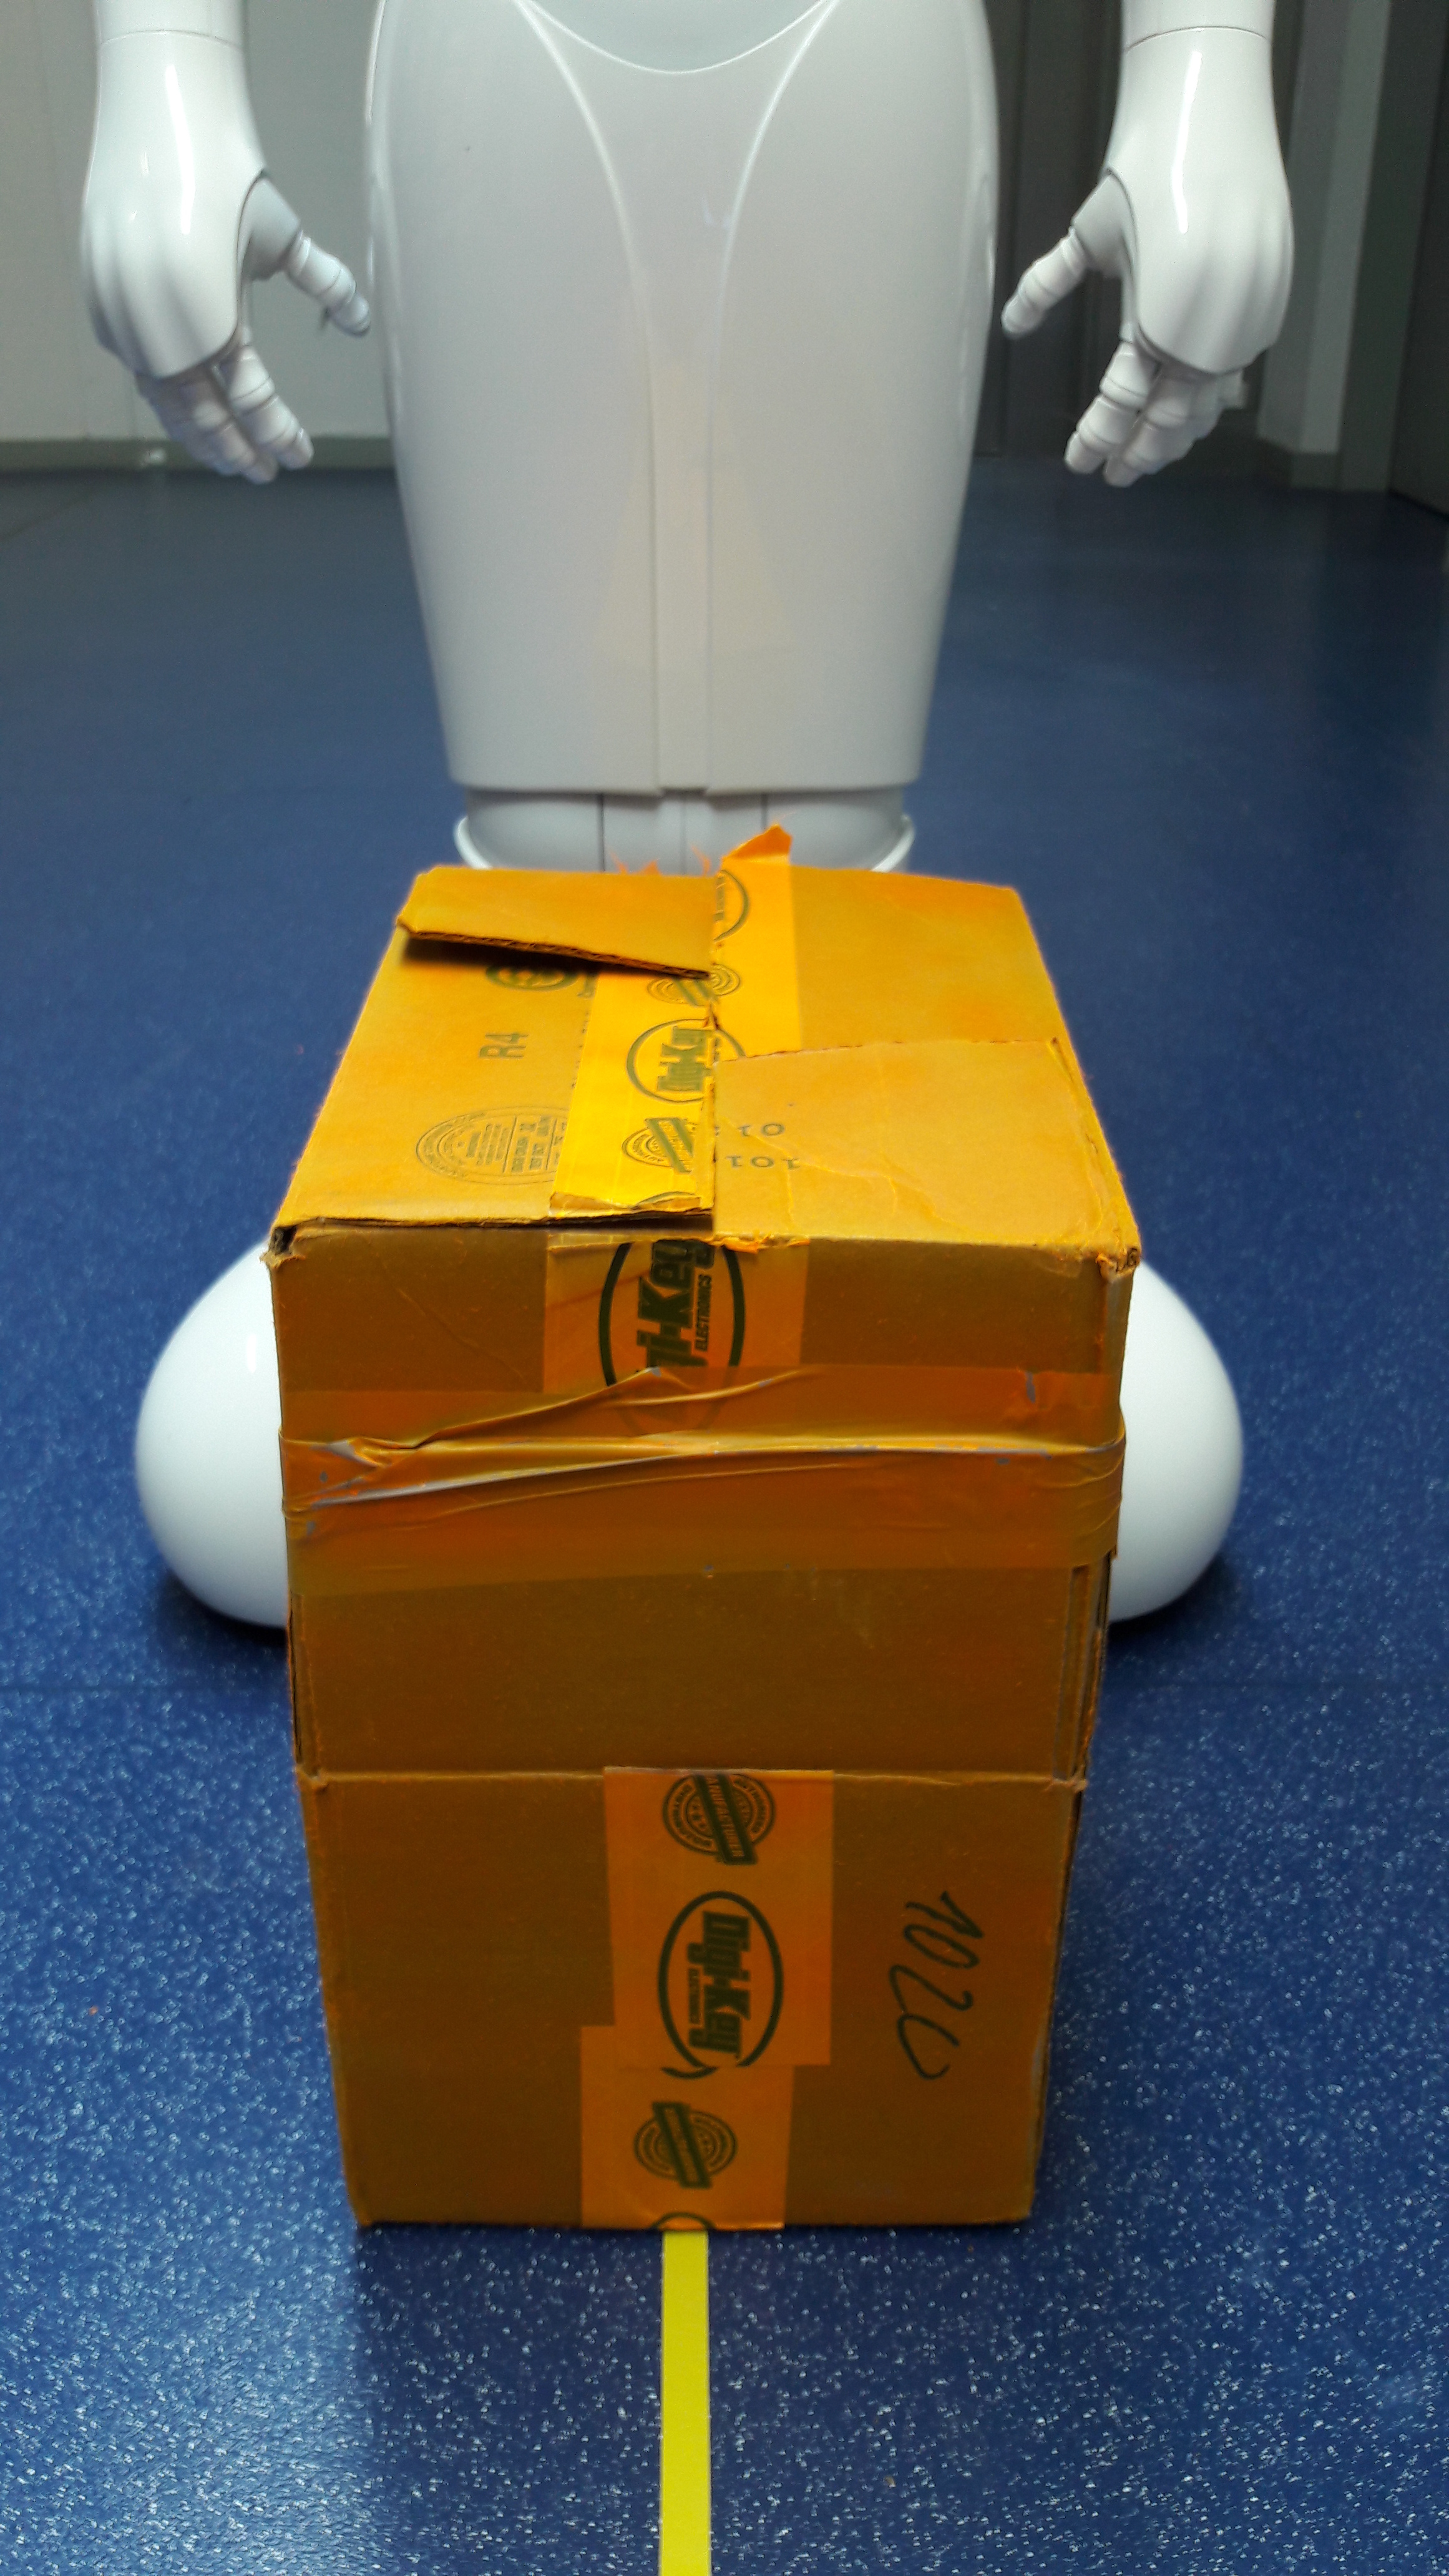
\includegraphics[width=\linewidth]{Experiment/01_init_front_close.jpg}
\caption{Front close angle} \label{fig:01_init_front_close}
\end{subfigure}\hspace*{\fill}
\begin{subfigure}{0.20\textwidth}
\includegraphics[width=\linewidth]{Experiment/01_init_front_wide.jpg}
\caption{Front wide angle} \label{fig:01_init_front_wide}
\end{subfigure}\hspace*{\fill}
\begin{subfigure}{0.20\textwidth}
\includegraphics[width=\linewidth]{Experiment/01_init_side_close.jpg}
\caption{Side close angle} \label{fig:01_init_side_close}
\end{subfigure}

\medskip

\begin{subfigure}{0.35\textwidth}
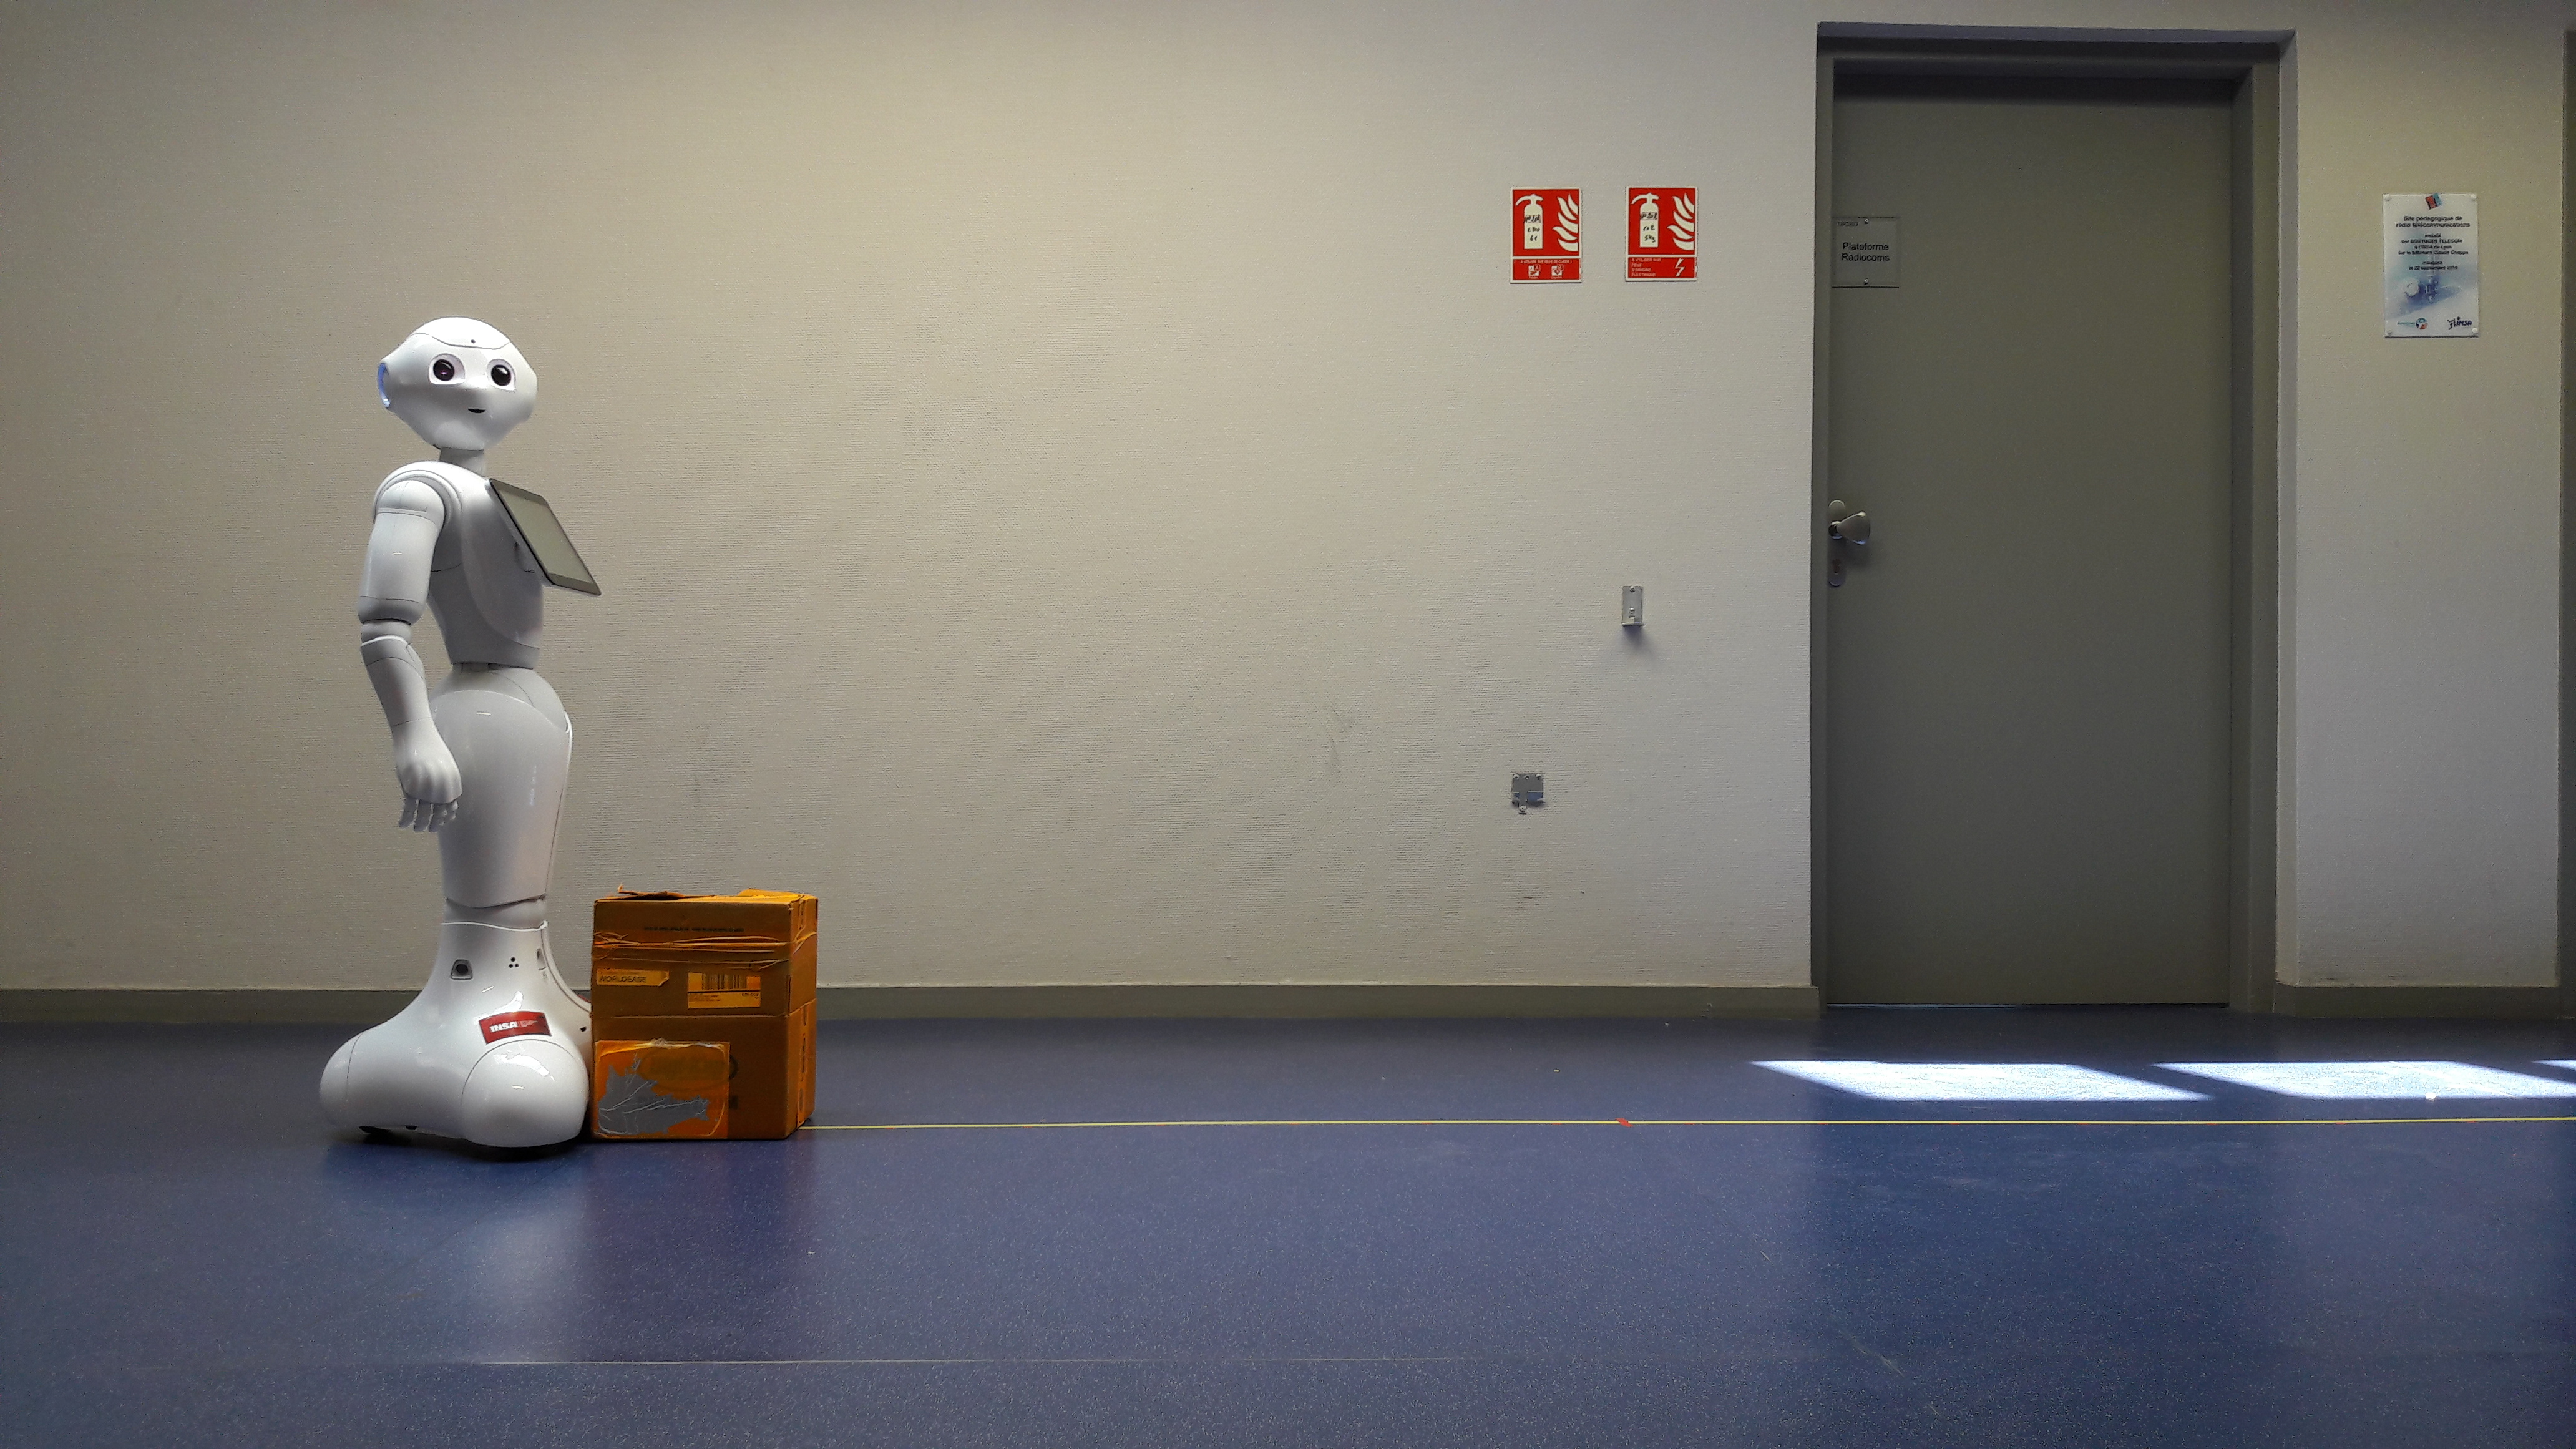
\includegraphics[width=\linewidth]{Experiment/01_init_side_wide.jpg}
\caption{Side wide angle} \label{fig:01_init_side_wide}
\end{subfigure}\hspace*{\fill}
\begin{subfigure}{0.35\textwidth}
\includegraphics[width=\linewidth]{Experiment/01_init_top.jpg}
\caption{Top close angle} \label{fig:01_init_top}
\end{subfigure}

\caption{Experimental setup example with a small cardboard box} \label{fig:experimental_setup}
\end{figure}

\paragraph{Results}

\paragraph{} After tests conducted on empty cardboard boxes of varied sizes (bigger or smaller than the robot's base), a chair with wheelcasters and an office trash can, we experimentally conclude that:
\begin{itemize}
  \item Pushing obstacles with wheelcasters without grasping nor adaptive procedures to compensate their drift, results in quick drifts from the robot's trajectory, because each wheelcaster generally has its own friction constraints, and even when all are manually orientated in the same direction, they rotate in an unpredictable way (Figures \ref{fig:03_init_top} and \ref{fig:03_end_top}).
  \item Light polygonal or round obstacles with an even distribution of mass (boxes and can), drift little if not at all from the robot's trajectory if the robot is placed so that its center faces the center of the side of the obstacle being pushed (the center of the circle for round obstacles). For the cardboard boxes, as long as the robot's span is within the span of the obstacle, little drift is produced from the robot's trajectory, but as soon as the robot's span overflows a little (Figures \ref{fig:02_init_front_wide} and \ref{fig:02_end_front_wide}), there is a significant drift (likely caused by the fact that it makes the robot start with only one contact point with the obstacle at the beginning).
\end{itemize}

\paragraph{Conclusion} Therefore, it is relatively safe to assume that always placing our robot at the middle of the obstacle's side for a push action will almost always produce the expected translation without significant drift.

\begin{figure}[H]

\begin{subfigure}{0.18\textwidth}
\includegraphics[width=\linewidth]{Experiment/03_init_top.jpg}
\caption{Initial top close angle of well-positioned robot and chair} \label{fig:03_init_top}
\end{subfigure}\hspace*{\fill}
\begin{subfigure}{0.18\textwidth}
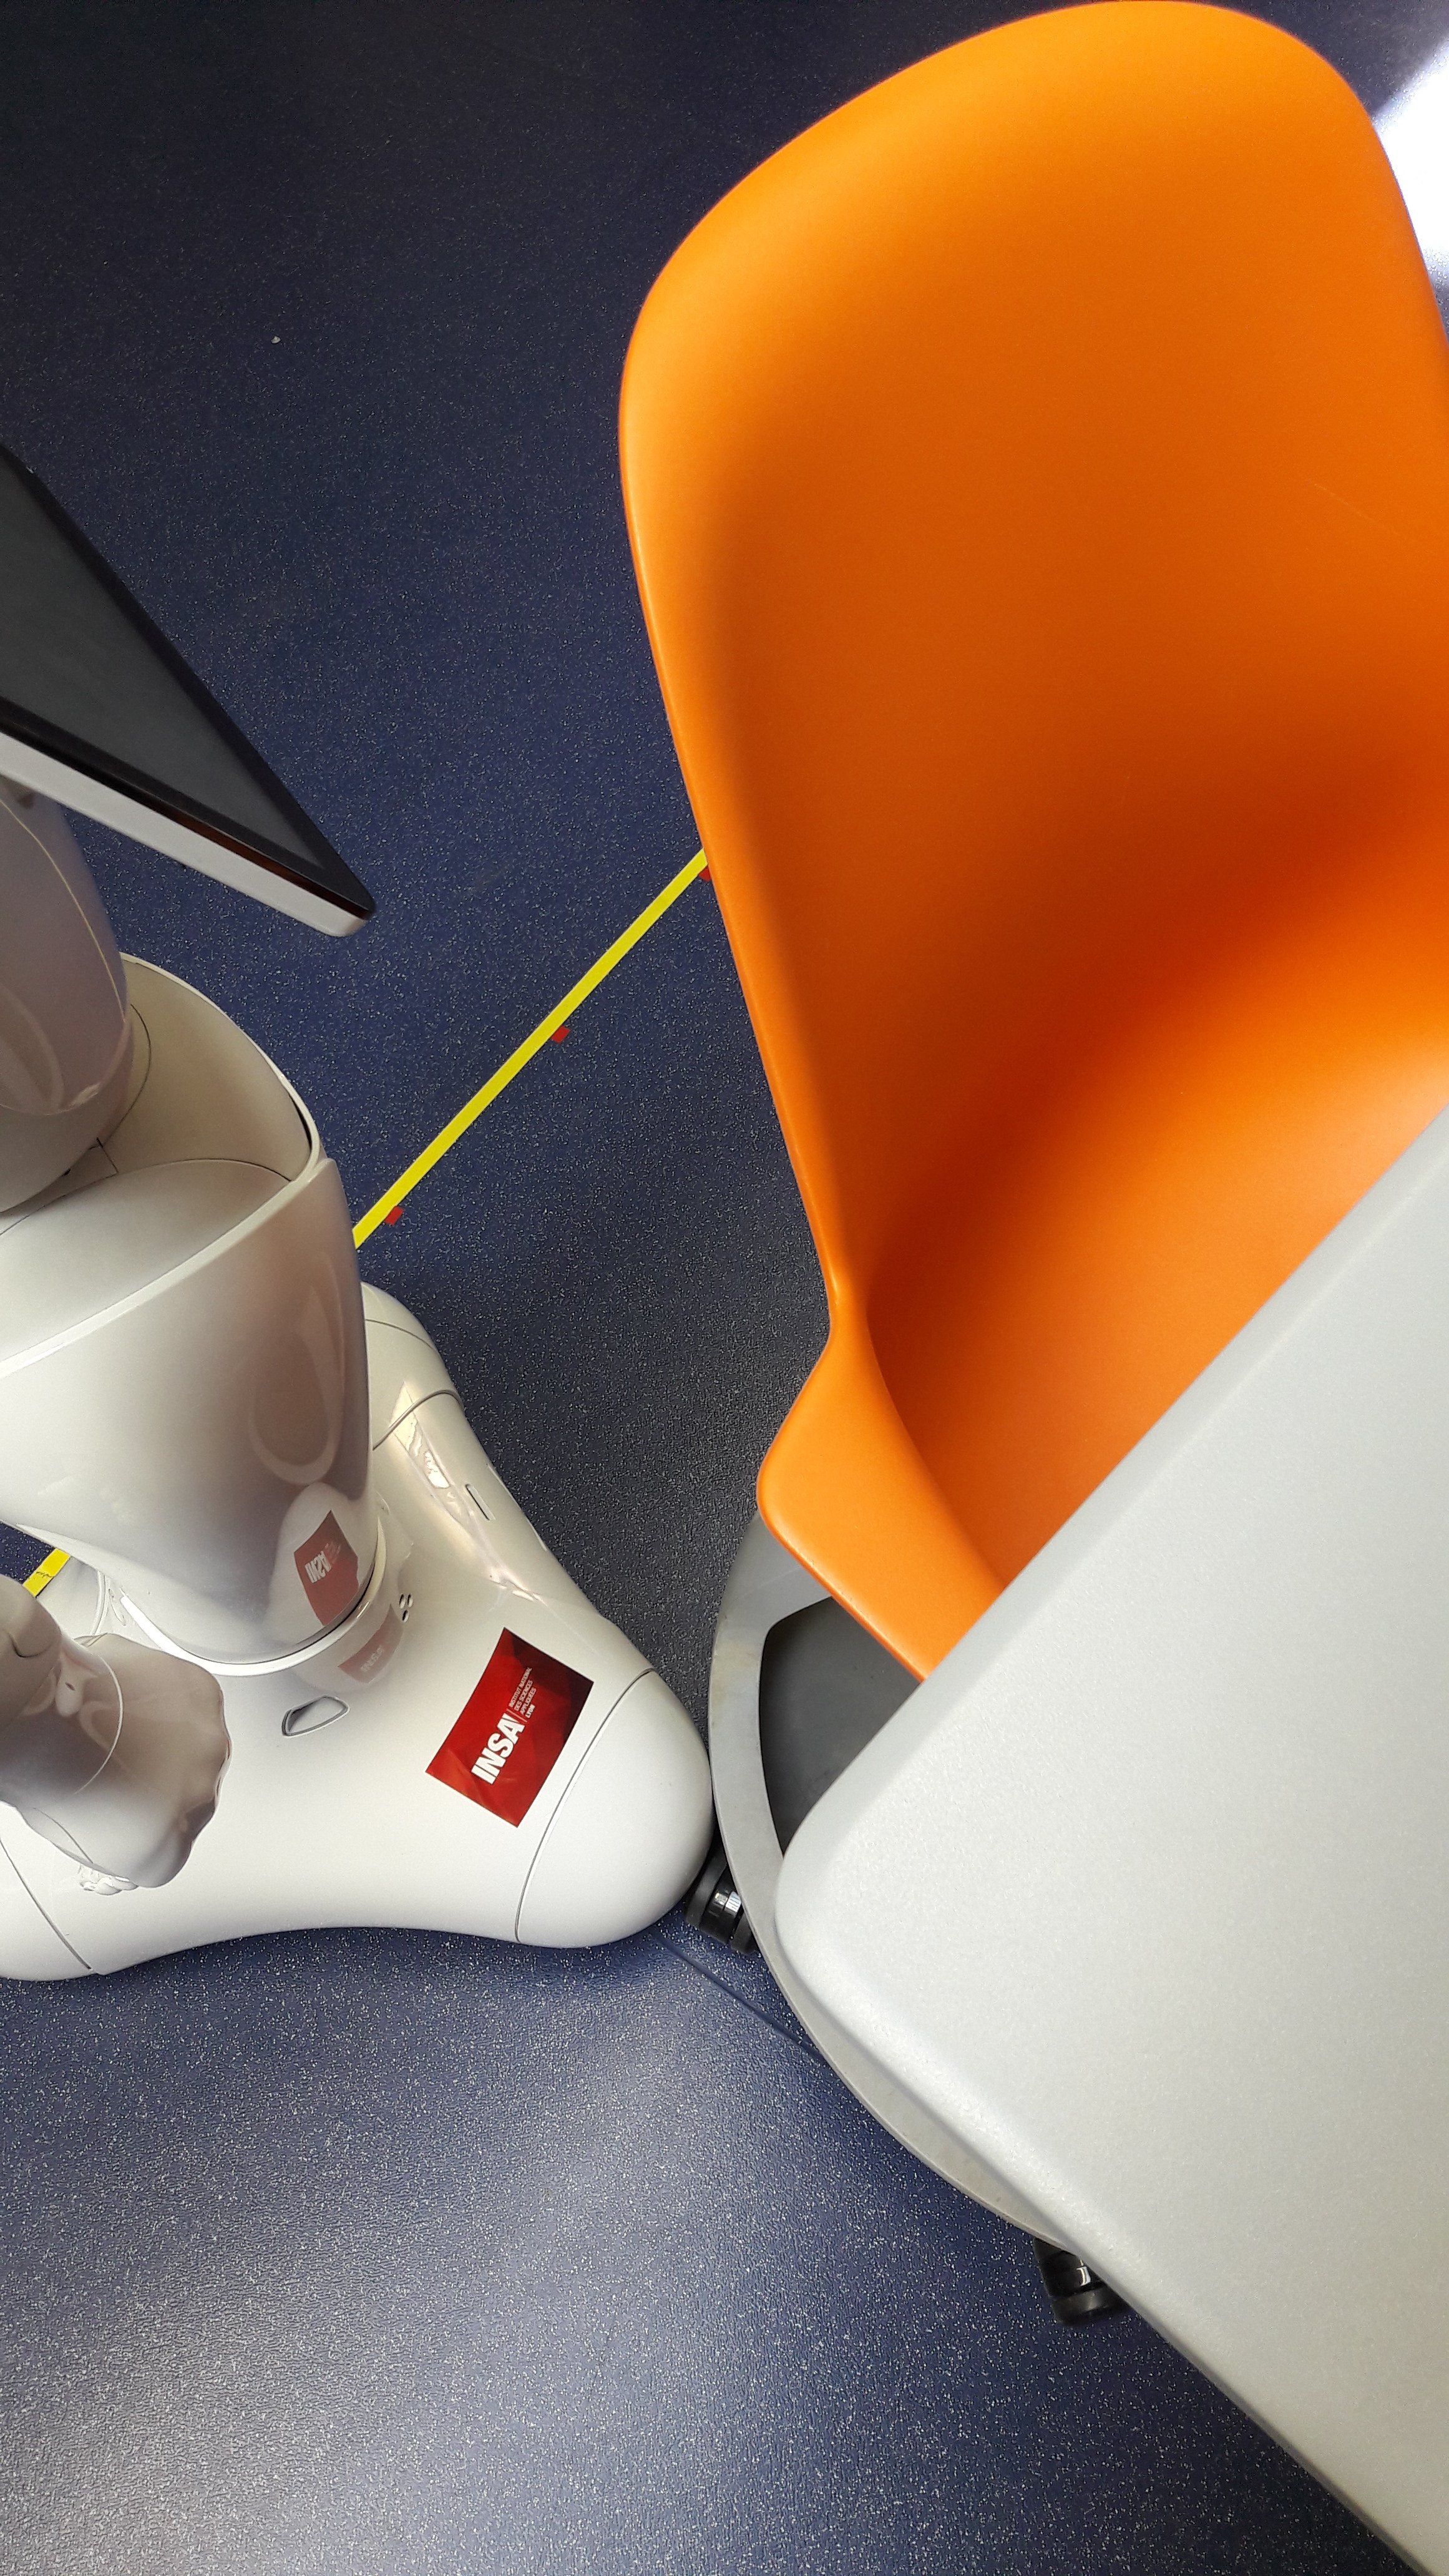
\includegraphics[width=\linewidth]{Experiment/03_end_top.jpg}
\caption{Final top close angle of the failed chair push attempt} \label{fig:03_end_top}
\end{subfigure}\hspace*{\fill}
\begin{subfigure}{0.18\textwidth}
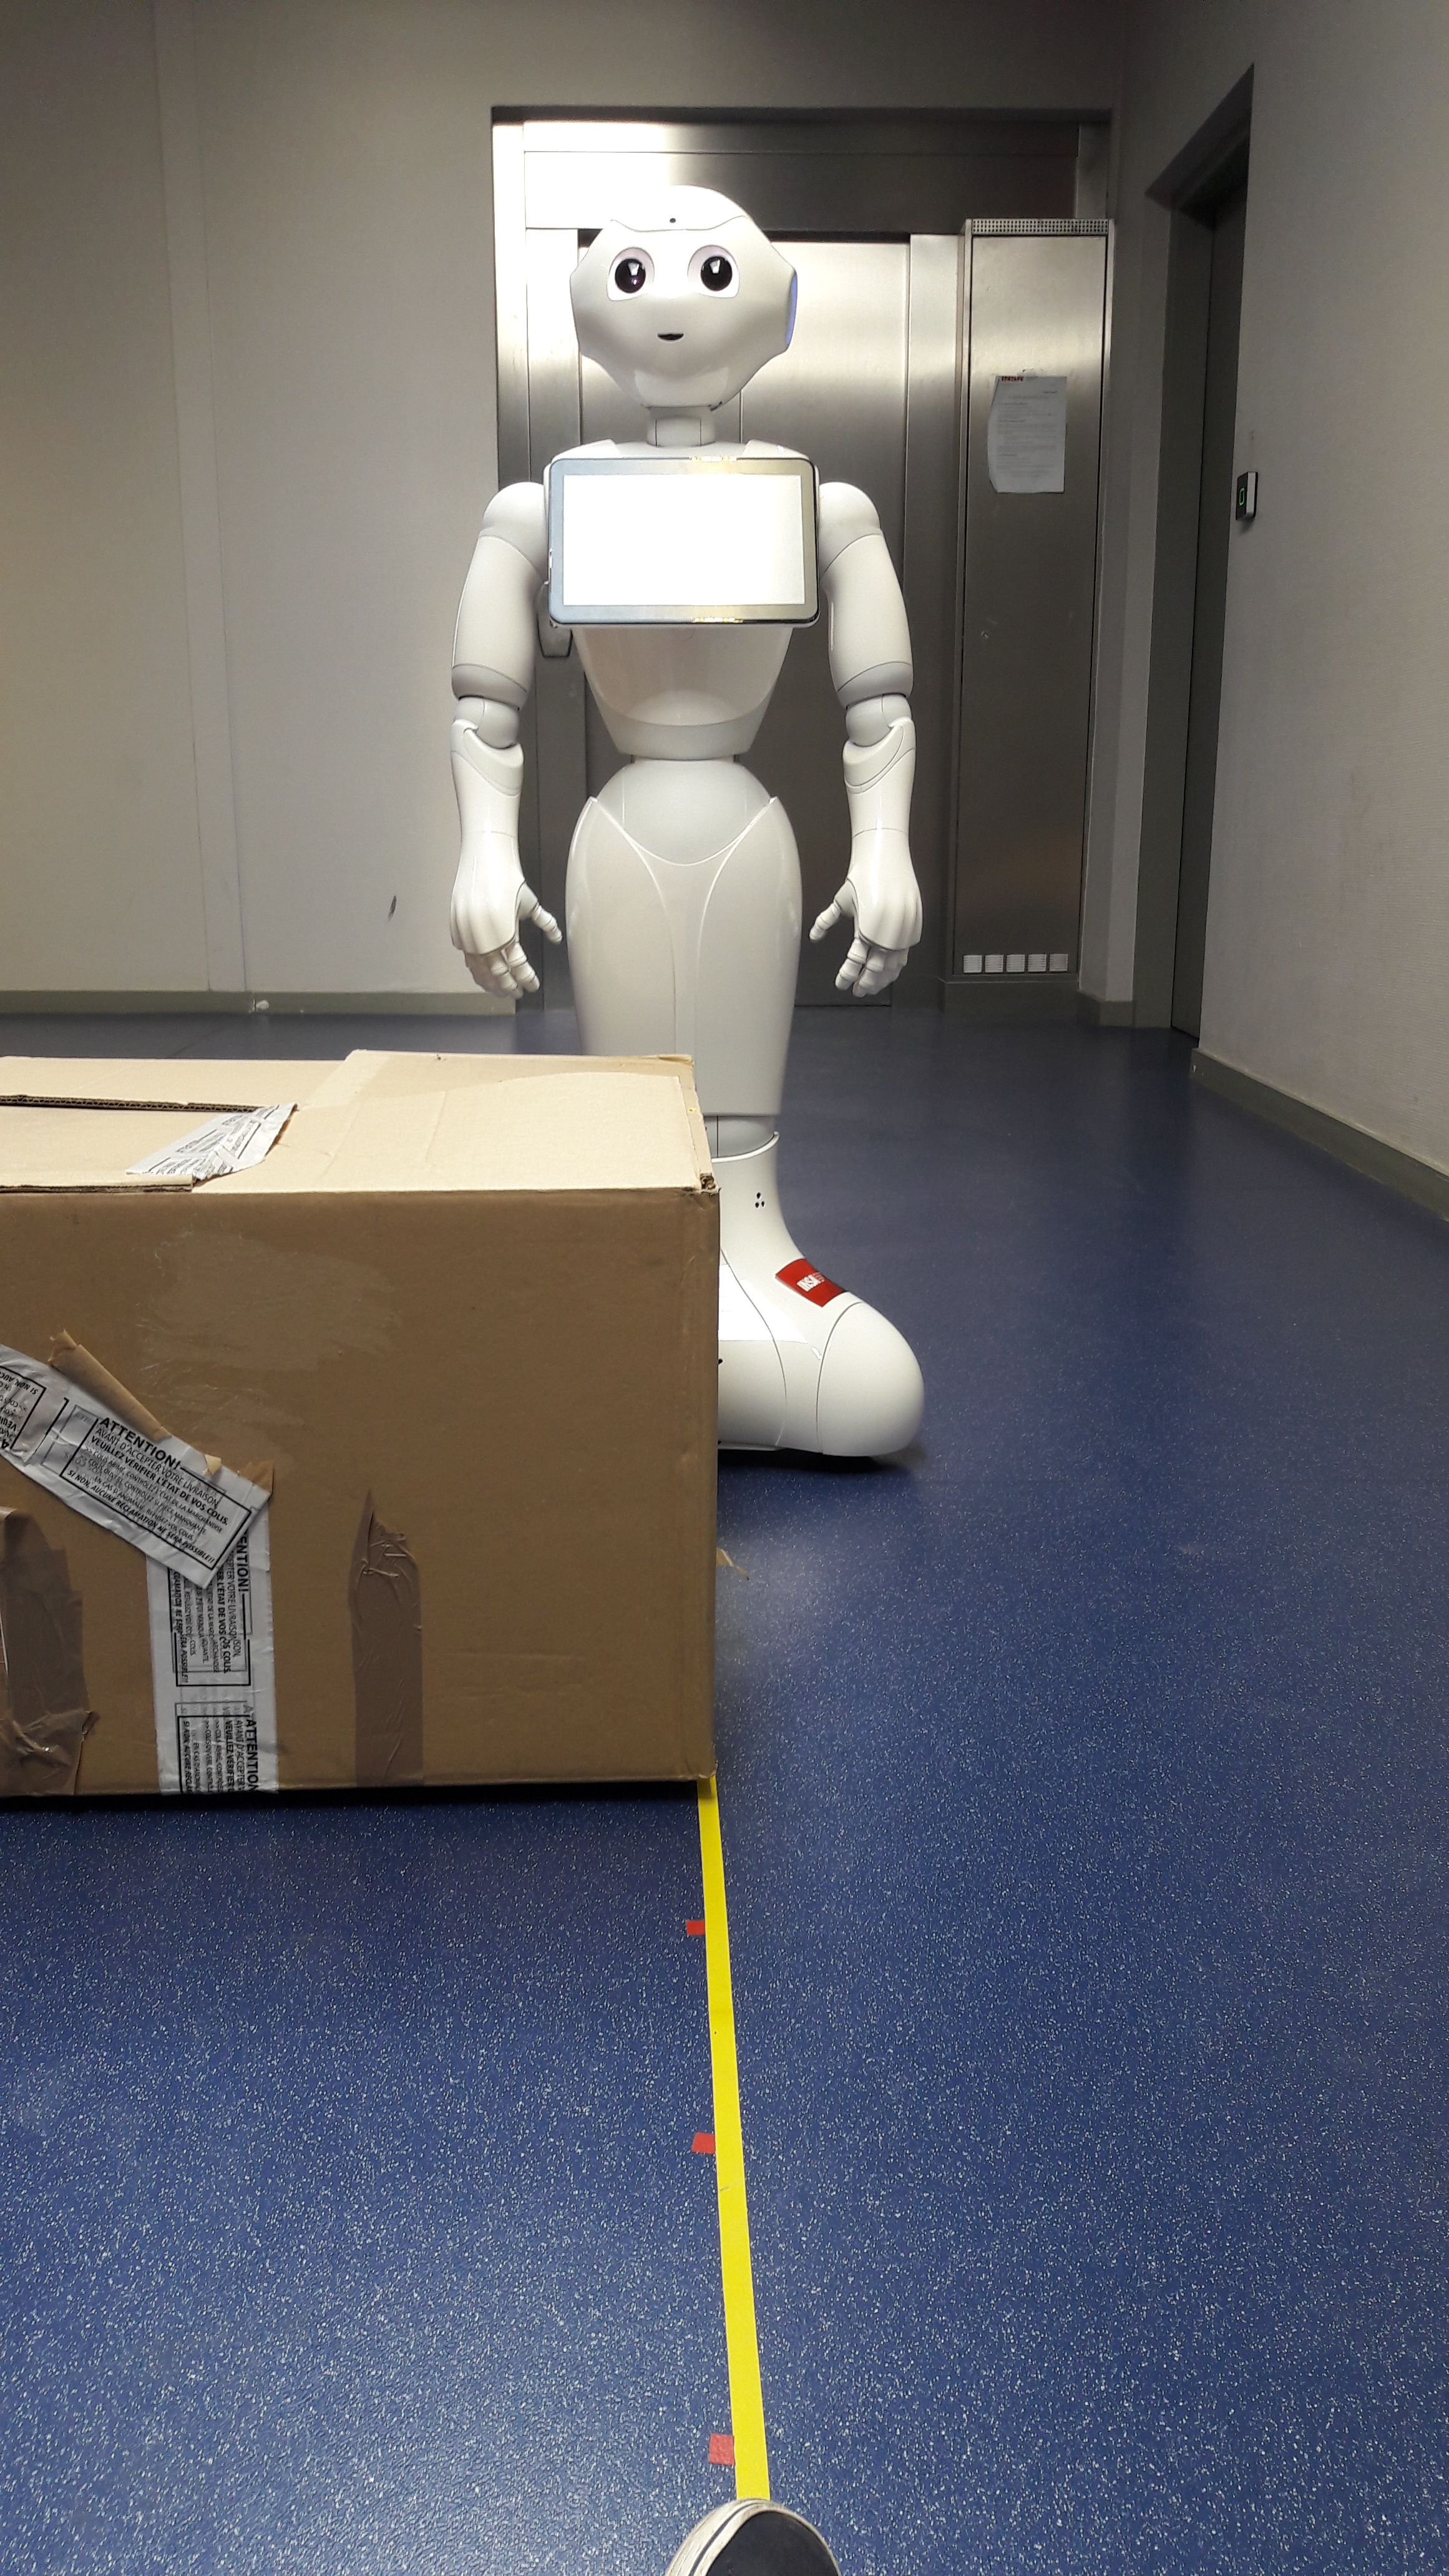
\includegraphics[width=\linewidth]{Experiment/02_init_front_wide.jpg}
\caption{Initial front wide angle of badly-positioned robot and box} \label{fig:02_init_front_wide}
\end{subfigure}\hspace*{\fill}
\begin{subfigure}{0.18\textwidth}
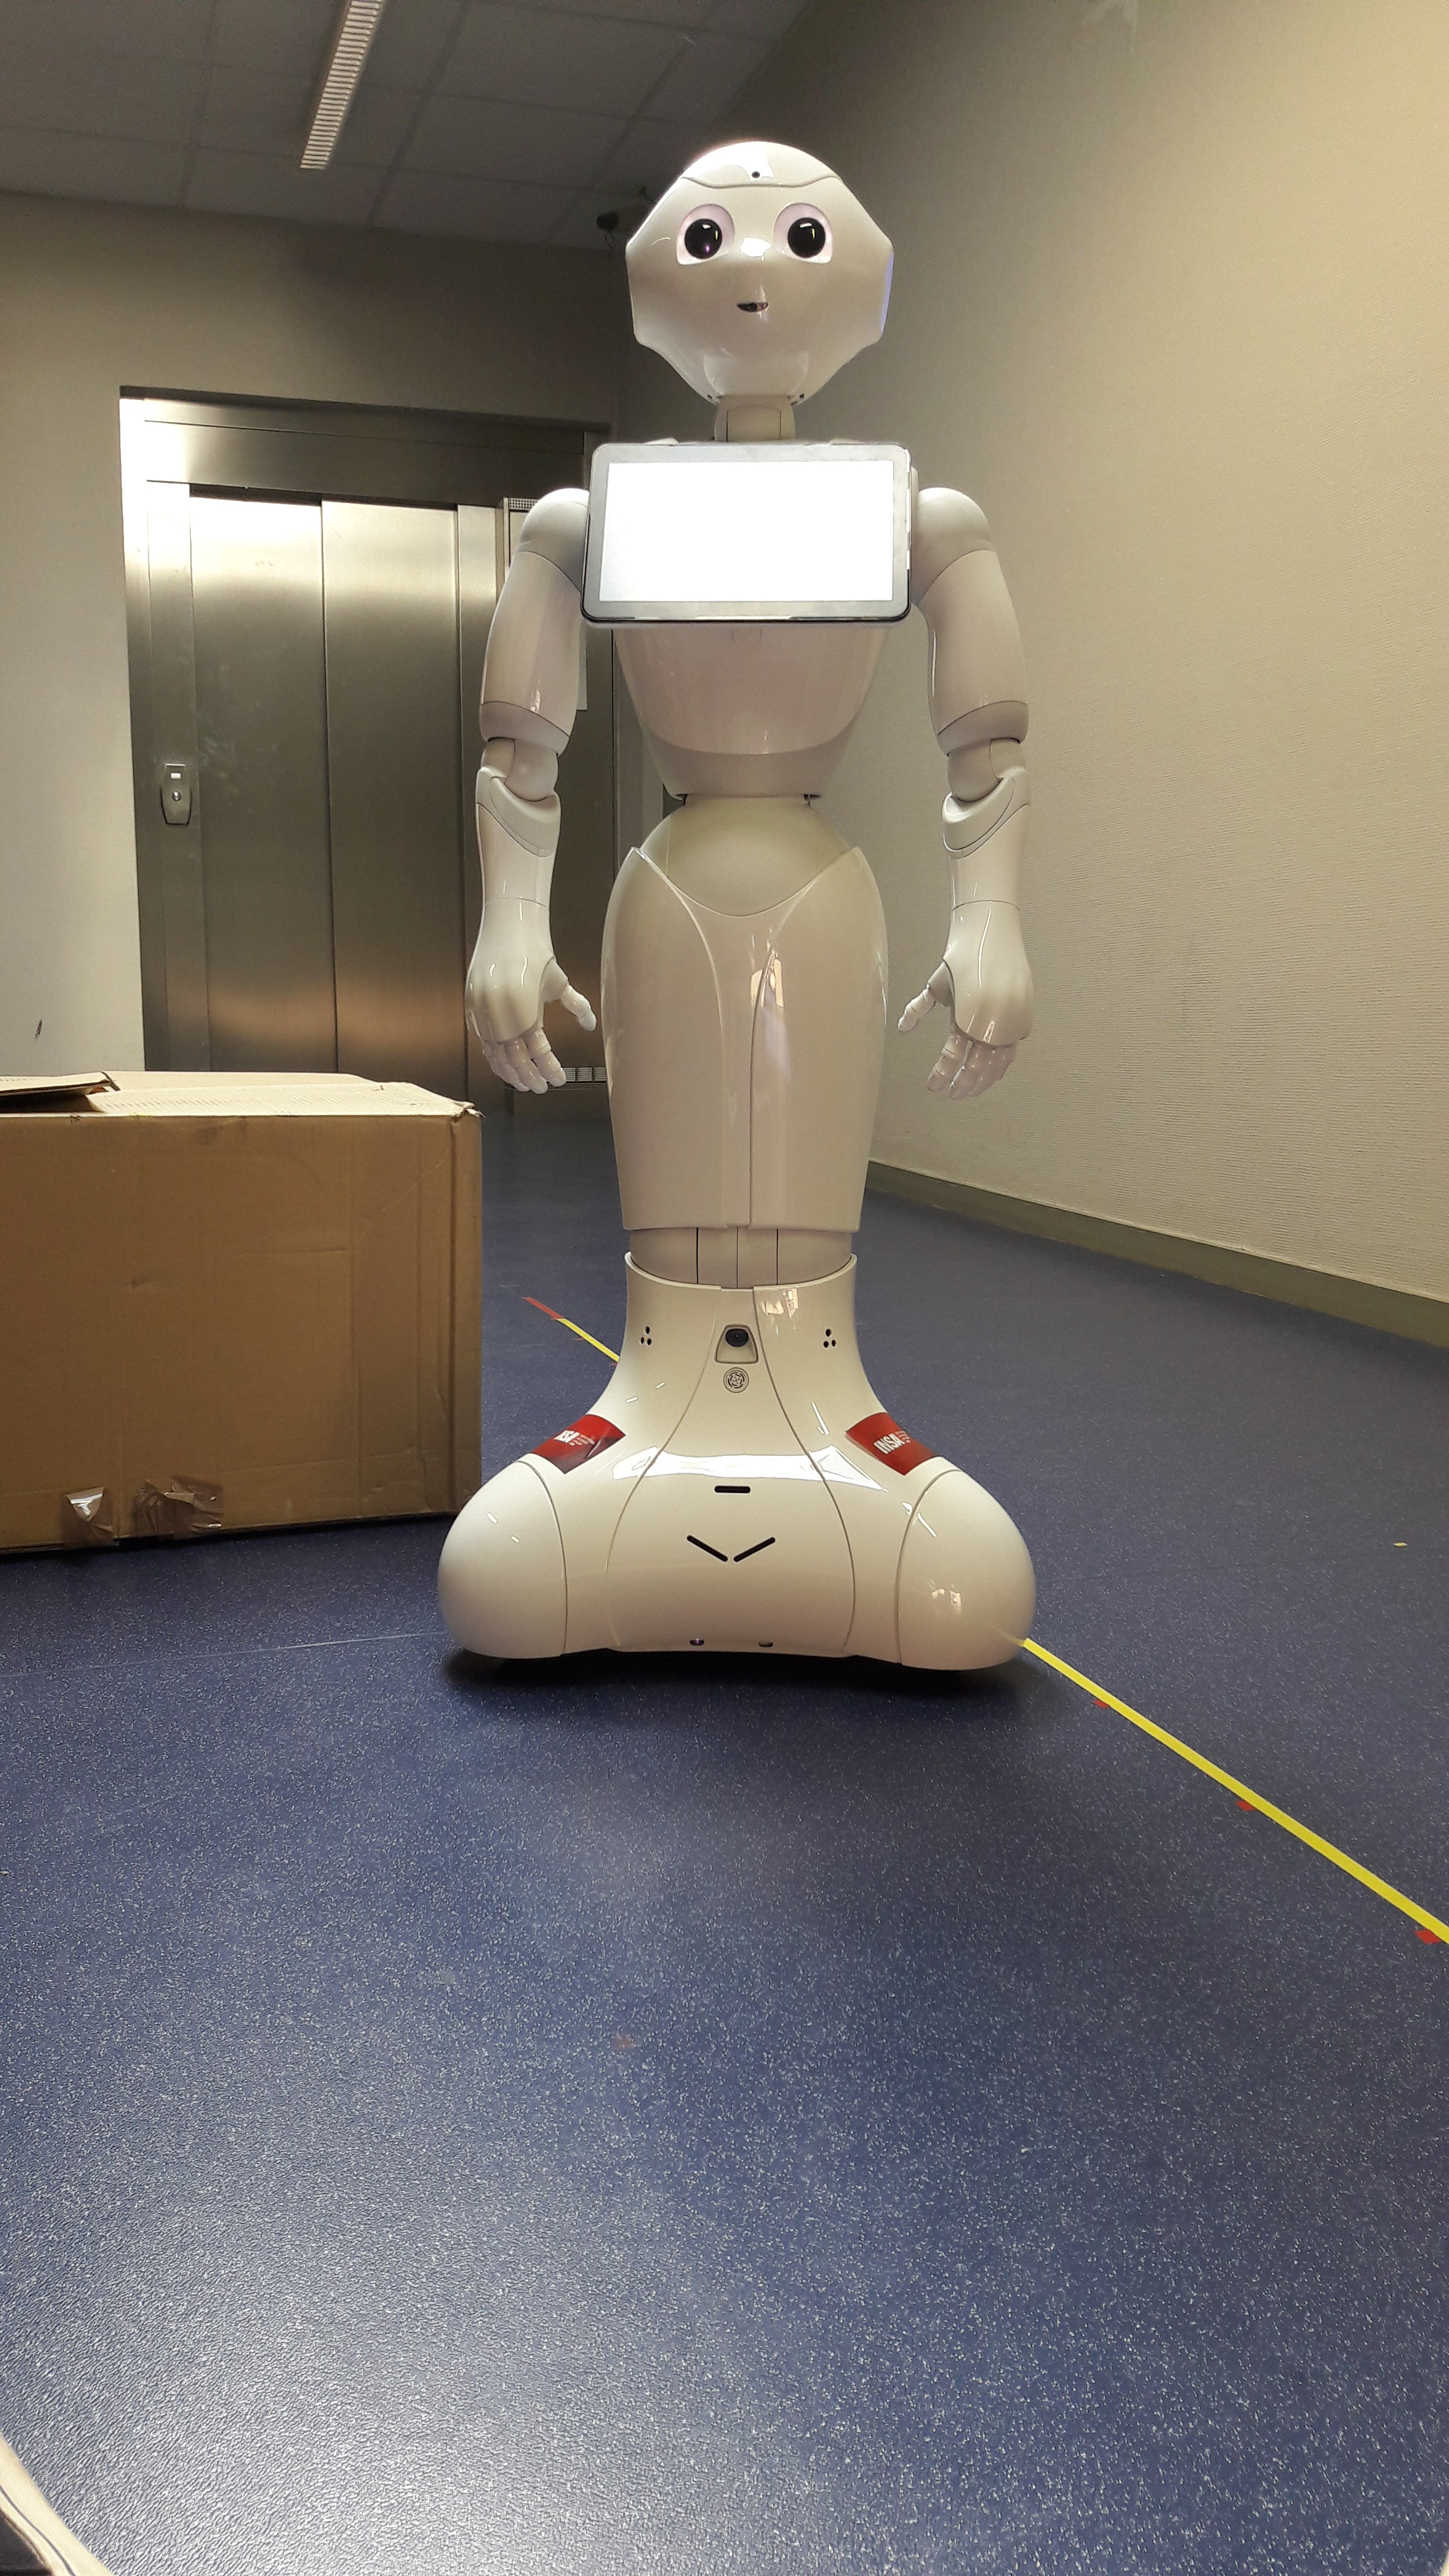
\includegraphics[width=\linewidth]{Experiment/02_end_front_wide.jpg}
\caption{Final front wide angle of the failed box push attempt} \label{fig:02_end_front_wide}
\end{subfigure}

\caption{Failed manipulation attempts with badly positioned robot and a carboard box, and with well-positioned robot and a chair with wheelcasters.} \label{fig:failed_attempts}
\end{figure}

\section{Simulation in a ROS-Standards compatible simulator}

\subsection{Simulator presentation}

\paragraph{} In order to test our propositions in Chapter \ref{Chapter4}, and validate our many improvements over the original algorithm formulation in Chapter \ref{Chapter3}, we developed a custom simulator based on ROS standards. By that, we mean that the simulator uses ROS standard message types\footnote{See ROS documentation page: \url{http://wiki.ros.org/common_msgs}}, to exchange data about the poses, observations of the robot, path to follow, ... This, in itself, reduces the gap to implement our propositions on a real robot (Pepper), since the only missing piece for a first implementation in the real world is an obstacle sensing identification component that would produce the data currently provided by our simulator (pointcloud of the obstacles geometry with each point identified with a specific obstacle id). The vizualition is done by RViz\footnote{See ROS documentation page: http://wiki.ros.org/rviz}(Figure \ref{fig:rviz}), the standard 3D visualizer for ROS, simply by listening to the messages exchanged by the program and the simulator and displaying them with its default visual components.

\paragraph{} It is to be noted that the optimality target for this implementation is at the moment only expressed in distance, but it is relatively trivial to express it in time or energy, by using the $move\_cost$ and $push\_cost$ currently present in the algorithm and passing them to the A* path finding subroutine.

\paragraph{} All the code and its execution instructions are available on the following repository: \\ \url{https://github.com/Xia0ben/namo_navigation} .

\begin{figure}[H]
\centering
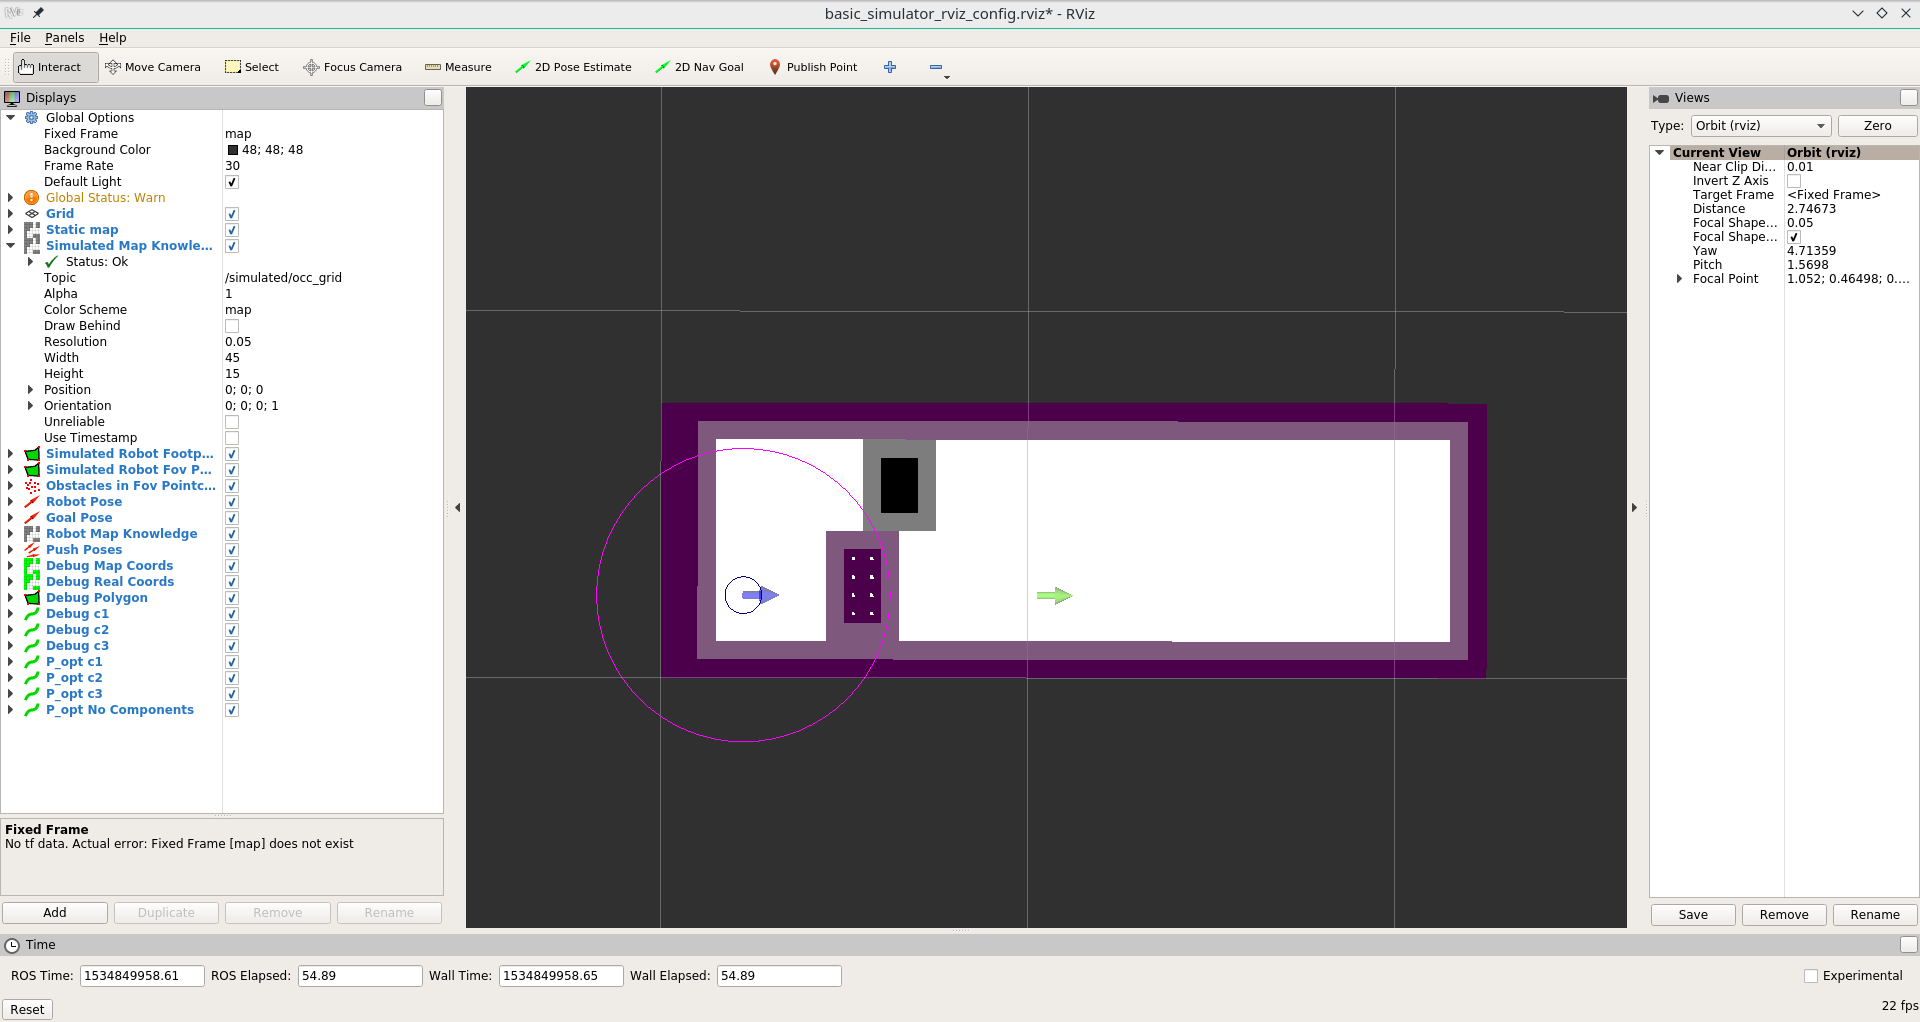
\includegraphics[width=14cm]{Figures/Simulation/rviz.png}
\caption{Rviz interface screenshot. On the left, we can see the visual components used and the message topics they listen to. In the center, we can see in real time the execution of the algorithm: the representations are explained in the following section \ref{simulation_results_subsection}.}
\label{fig:rviz}
\end{figure}

\subsection{Simulation results}\label{simulation_results_subsection}

\paragraph{} At the time of the writing of this report, we were only able to implement the algorithm and the necessary simulation code for the solution presented in section \ref{discussion_hypotheses_section} (and corresponding algorithms \ref{alg:03-custom-basicmods-makeandexecuteplan}, \ref{alg:02-levihn-makeplan} and \ref{alg:03-custom-basicmods-planforobstacle}), but not the three propositions that build upon it. This still allowed us to validate all comments and improvements made in Chapter \ref{Chapter3} and in the first section of Chapter \ref{Chapter4}. Below are a few figures (\ref{fig:simulation}) showing a test case in a corridor with two obstacles.

\paragraph{} Figure \ref{fig:simulation_01} represents the static obstacles that \textbf{never change} (walls). Figure \ref{fig:simulation_02} also represents the yet unknown obstacles (the bottom one is unmovable, the top one is movable). Figure \ref{fig:simulation_03} is our initial robot configuration. The robot is geometrically represented by a little blue circle and a blue arrow for its orientation, and it's field of vision (represented by the pink circle) allows it to detect the point cloud (white point) that represents the bottom obstacle (known environment to the robot is represented by the purple shades).

\paragraph{} In Figure \ref{fig:simulation_04}, the robot starts by considering a plan ignoring all obstacles, except the static ones (because we made the hypothesis that it knows about them). Then, in Figure \ref{fig:simulation_05}, it takes into account its current knowledge of the environment to see that its previous best plan is invalid and sets its new best plan as the one that avoids the obstacle. In Figure \ref{fig:simulation_06}, the robot evaluates the bottom obstacle and finds a better plan pushing the obstacle than the one avoiding it, and starts executing this plan in Figure \ref{fig:simulation_07}, where we see that is starts detecting the shape of the top obstacle, only to realize in \ref{fig:simulation_08} that the obstacle won't budge. Therefore, it invalidates the current plan, and computes a new one (seen in Figure \ref{fig:simulation_09}) that implies moving the top obstacle directly, since no plan avoiding the two obstacles could be found. In Figures \ref{fig:simulation_10} and \ref{fig:simulation_11}, the robot moves the top obstacle, to finally reach its goal in Figure \ref{fig:simulation_12}.

\begin{figure}[H]

\begin{subfigure}{0.48\textwidth}
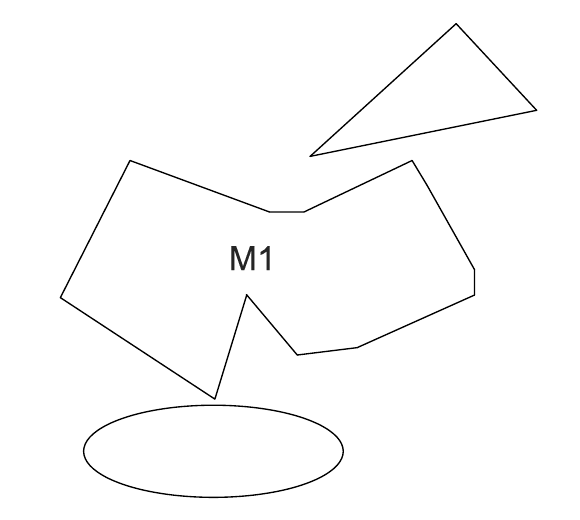
\includegraphics[width=\linewidth]{Simulation/01.png}
\caption{} \label{fig:simulation_01}
\end{subfigure}\hspace*{\fill}
\begin{subfigure}{0.48\textwidth}
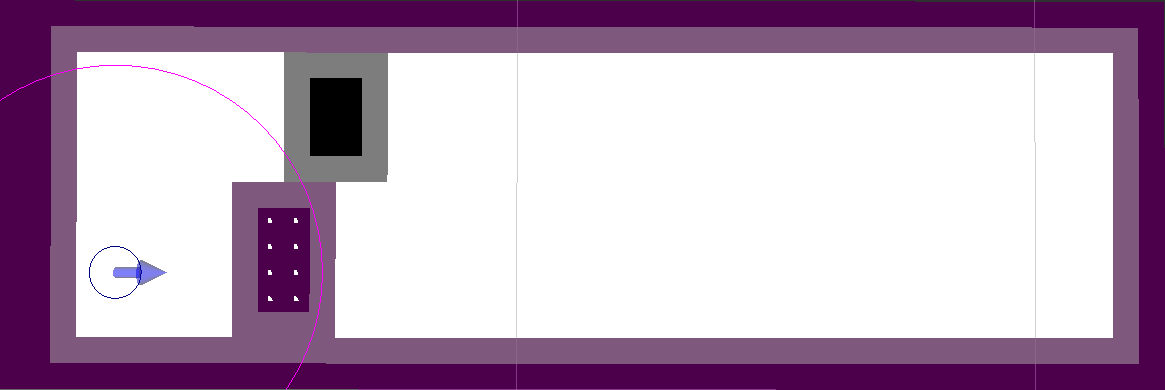
\includegraphics[width=\linewidth]{Simulation/02.png}
\caption{} \label{fig:simulation_02}
\end{subfigure}

\medskip

\begin{subfigure}{0.48\textwidth}
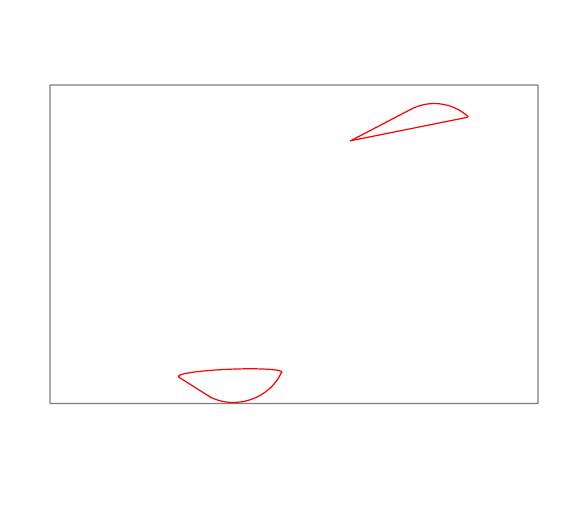
\includegraphics[width=\linewidth]{Simulation/03.png}
\caption{} \label{fig:simulation_03}
\end{subfigure}\hspace*{\fill}
\begin{subfigure}{0.48\textwidth}
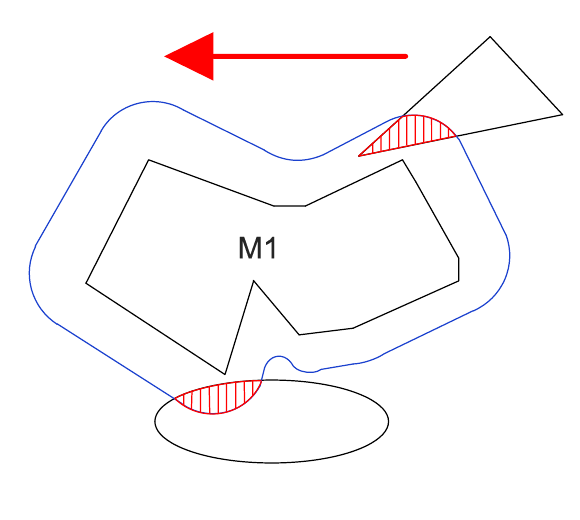
\includegraphics[width=\linewidth]{Simulation/04.png}
\caption{} \label{fig:simulation_04}
\end{subfigure}

\medskip

\begin{subfigure}{0.48\textwidth}
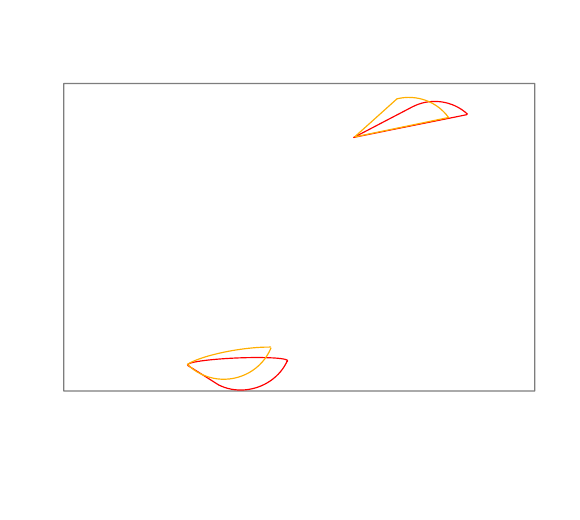
\includegraphics[width=\linewidth]{Simulation/05.png}
\caption{} \label{fig:simulation_05}
\end{subfigure}\hspace*{\fill}
\begin{subfigure}{0.48\textwidth}
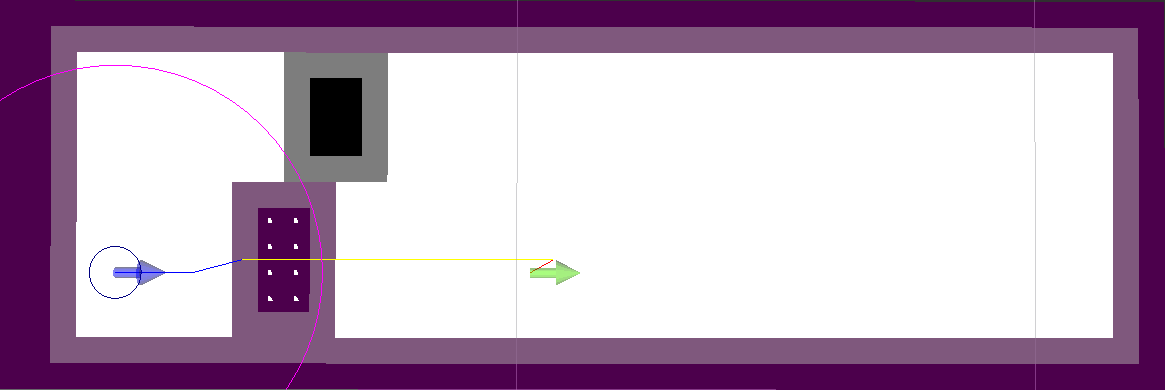
\includegraphics[width=\linewidth]{Simulation/06.png}
\caption{} \label{fig:simulation_06}
\end{subfigure}

\medskip

\begin{subfigure}{0.48\textwidth}
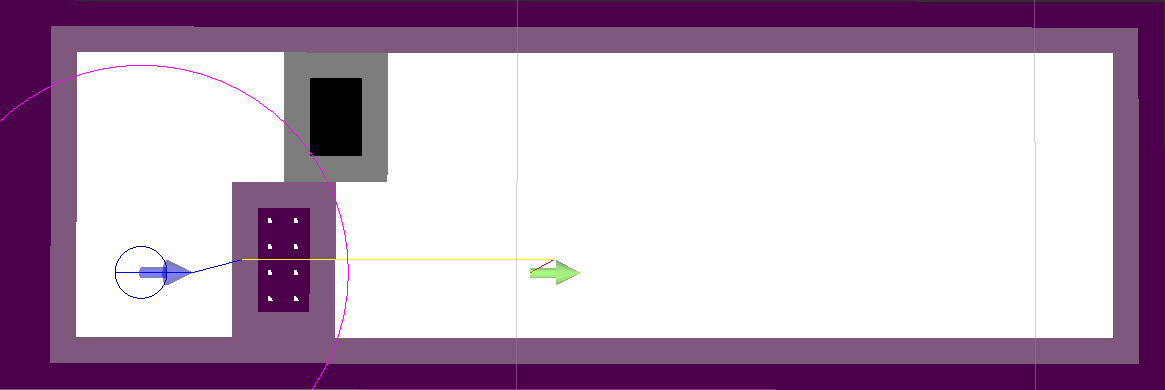
\includegraphics[width=\linewidth]{Simulation/07.png}
\caption{} \label{fig:simulation_07}
\end{subfigure}\hspace*{\fill}
\begin{subfigure}{0.48\textwidth}
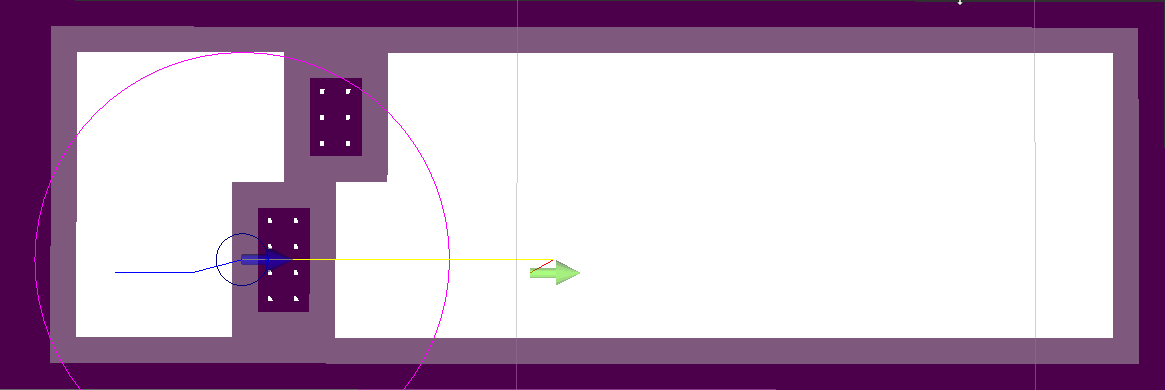
\includegraphics[width=\linewidth]{Simulation/08.png}
\caption{} \label{fig:simulation_08}
\end{subfigure}

\medskip

\begin{subfigure}{0.48\textwidth}
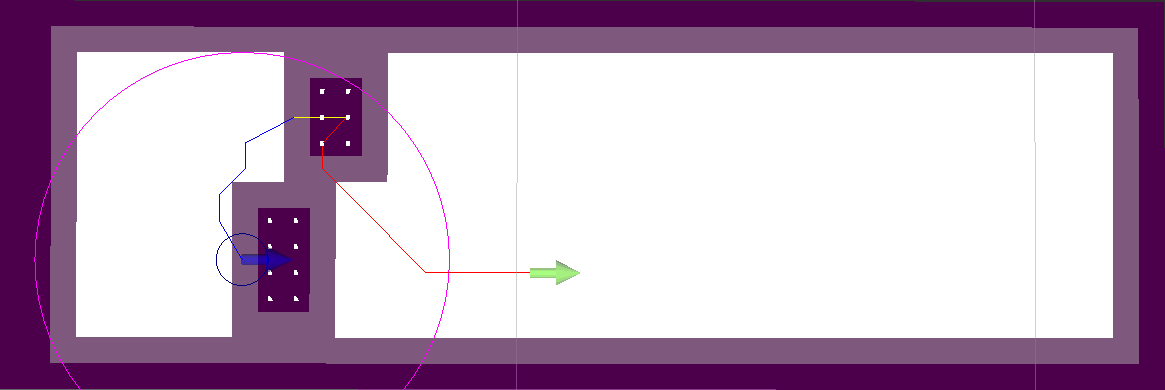
\includegraphics[width=\linewidth]{Simulation/09.png}
\caption{} \label{fig:simulation_09}
\end{subfigure}\hspace*{\fill}
\begin{subfigure}{0.48\textwidth}
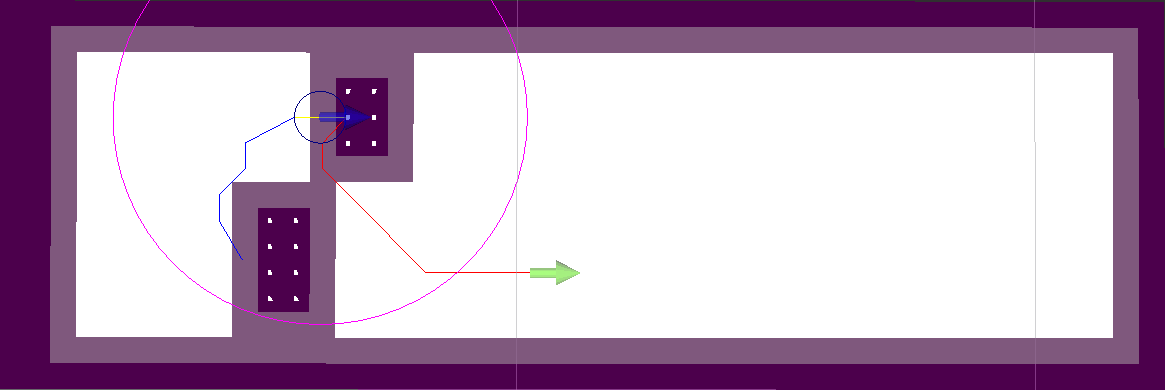
\includegraphics[width=\linewidth]{Simulation/10.png}
\caption{} \label{fig:simulation_10}
\end{subfigure}

\medskip

\begin{subfigure}{0.48\textwidth}
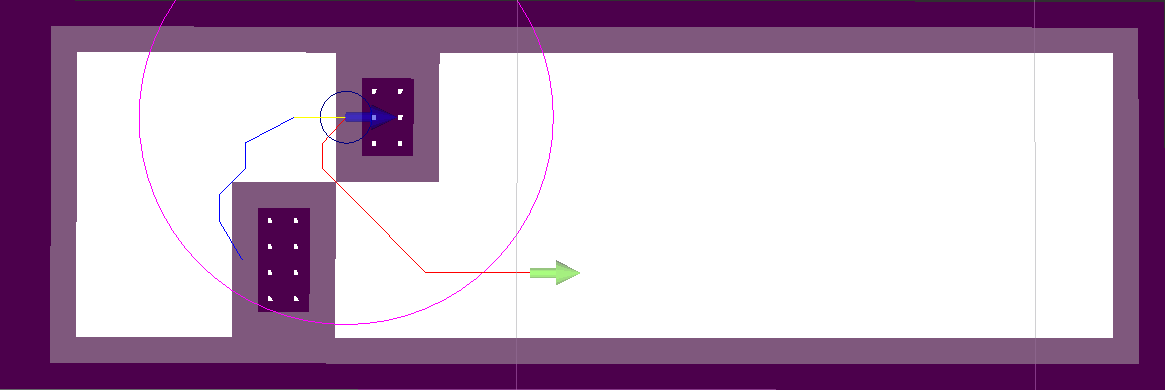
\includegraphics[width=\linewidth]{Simulation/11.png}
\caption{} \label{fig:simulation_11}
\end{subfigure}\hspace*{\fill}
\begin{subfigure}{0.48\textwidth}
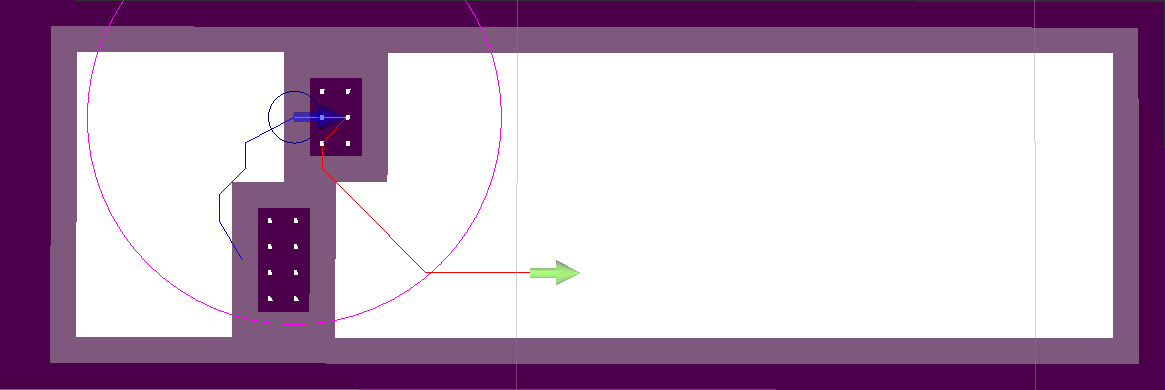
\includegraphics[width=\linewidth]{Simulation/12.png}
\caption{} \label{fig:simulation_12}
\end{subfigure}

\caption{Simple simulation in a corridor with a movable (top one) and an unmovable (bottom one) obstacles with our algorithm as presented in section \ref{discussion_hypotheses_section}. Our representations are explained in the previous paragraphs.} \label{fig:simulation}
\end{figure}
